\chapter{换一种消元顺序：二维 Spline2D}
\begin{notebox}
\textbf{目标}\quad 理解块三对角系统，验证同一最小 jerk 问题的系数与梯度，实测性能。\\
\textbf{先修}\quad 第 14、15 章；本章固定二维五次，不扩展到任意阶通用框架。
\end{notebox}

\section{先固定问题，再比较实现}
\begin{lstlisting}[language=bash]
ros2 run motion2d spline_demo tmp/ch16_spline
bash scripts/benchmark_ch16.sh
/usr/bin/python3 scripts/plot_ch16_spline.py
\end{lstlisting}
第一条无需下载。第二条是可选上游对照，使用
\href{https://github.com/Bziyue/SplineTrajectory}{SplineTrajectory} 的 QuinticSplineND<2>，固定版本为
\texttt{126525e49a43b0548bc6960e4979dd6b6258f289}。
上游为 MIT 许可证；对照脚本只在临时目录读取它，课程核心独立实现。
本章的 Spline2D 和上一章 MINCO 解决\textbf{同一个 clamped 最小 jerk 问题}：
相同首尾 p/v/a、内部位置和正时长，结果应相同。它不是另一条曲线，也不是把路点当 B-spline 控制点。

\section{未知数改为连接点的速度与加速度}
单段边界状态写为 $W_i=[p_i,v_i,a_i,p_{i+1},v_{i+1},a_{i+1}]^T$，每行有 x/y 两列。
第十四章已能从边界状态求六个系数，因此存在 $C_i=E_i(T_i)W_i$。
用单位边界依次调用 interpolateQuintic，可以直接构造 $E_i$ 的六列；无需初学者先抄一大组公式。
代入 jerk 二次型：
\begin{equation}
 J_i=\operatorname{tr}(W_i^TR_iW_i),\qquad R_i=E_i^TQ_iE_i.
\end{equation}
所有位置固定，首尾 v/a 固定，只有内部 $z_k=[v_k,a_k]^T$ 待求。
每段只含相邻两个节点，所以驻点条件形成对称块三对角系统：
\begin{equation}
 \begin{bmatrix}H_0&B_1^T&0\\B_1&H_1&B_2^T\\0&B_2&H_2\end{bmatrix}
 \begin{bmatrix}z_0\\z_1\\z_2\end{bmatrix}
 =\begin{bmatrix}r_0\\r_1\\r_2\end{bmatrix}.
\end{equation}
每个块为 $2\times2$，右端项有 x/y 两列。这是结构示例，实际块数为 $N-1$。
从各段 $R_i$ 取出对应 v/a 行列相加，已知位置和边界贡献移至右侧。

\clearpage
\section{一个块接一个块消元}
令 $D_0=H_0$，依次计算
\begin{equation}
 L_i=B_iD_{i-1}^{-1},\qquad D_i=H_i-L_iB_i^T.
\end{equation}
先解下三角，再解对角块，最后回代。每步固定规模，内存与时间随段数线性增长。
代码只对 $2\times2$ 正定块用 Cholesky 求解两个单位右端，缓存其逆作用；未显式求整张大矩阵的逆。
\lstinputlisting[language=C++,linerange={spline_blocks_begin-spline_blocks_end},
 includerangemarker=false]{../ros2_ws/src/motion2d/src/trajectory/spline2d.cpp}
得到所有节点 v/a 后，再经 $E_iW_i$ 还原为通用五次轨迹。
非正时长、维度不匹配、非有限数值或非正定分解均明确失败。任意悬殊时长仍可能损害浮点精度。

\section{能量梯度可以直接看边界}
第十五章分部积分给出的边界项也能用于梯度。内部位置的导数为两段第五阶导数之差：
\begin{equation}
 \frac{dJ}{dq_i}=2\left(p_{i-1}^{(5)}(T_{i-1})-p_i^{(5)}(0)\right).
\end{equation}
每段时长导数可在该段起点计算：
\begin{equation}
 \frac{dJ}{dT_i}=-\|p_i'''\|^2+2p_i''''\cdot p_i''-2p_i^{(5)}\cdot p_i'.
\end{equation}
这是固定端点、路点的\textbf{完整}导数；最优内部导数的变化因驻点条件消去。
把起点导数代成 $v=c_1,a=2c_2,j=6c_3,s=24c_4,p^{(5)}=120c_5$：
\lstinputlisting[language=C++,linerange={spline_energy_gradient_begin-spline_energy_gradient_end},
 includerangemarker=false]{../ros2_ws/src/motion2d/src/trajectory/spline2d.cpp}
该专用路径无需额外伴随。若加入 ESDF 等其他代价，仍需下一节的一般传播。

\clearpage
\section{任意代价的伴随如何复用块分解}
记未知内部导数为 $z$，其能量驻点条件为 $F(z,q,T)=0$，且 $F_z=H$。
给定系数偏导 $G_i$，先计算边界偏导 $E_i^TG_i$，累加得到 $K_z$。
再解 $H\lambda=K_z$，因此
\begin{equation}
 dK=K_q\,dq+K_T\,dT-\lambda^T(F_q\,dq+F_T\,dT).
\end{equation}
这里 $K_q,K_T$ 是固定 $z$ 的直接偏导。propagate 复用构造时的块分解求伴随。
为了计算 $E_T$，令 $M(T)C=W$ 为六个端点条件；由 $E=M^{-1}$ 得
$E_T=-EM_TE$。$M_T$ 只有末端三行非零，分别是速度、加速度、jerk 基函数。
然后对 $R=E^TQE$ 用乘积法则；这几步均为每段固定大小矩阵，仍是线性复杂度。

\section{误差验收与本机计时}
测试固定 seed=1616，1--12 段、非零边界 v/a、不同正时长。
系数与 MINCO 的相对误差要求低于 $10^{-9}$；MINCO 已另与独立密集 KKT 对照。
解析能量梯度与通用伴随交叉检查；含速度/加速度软惩罚的一般传播用 $10^{-5}$ 中心差分检查。

\begin{figure}[!ht]
\centering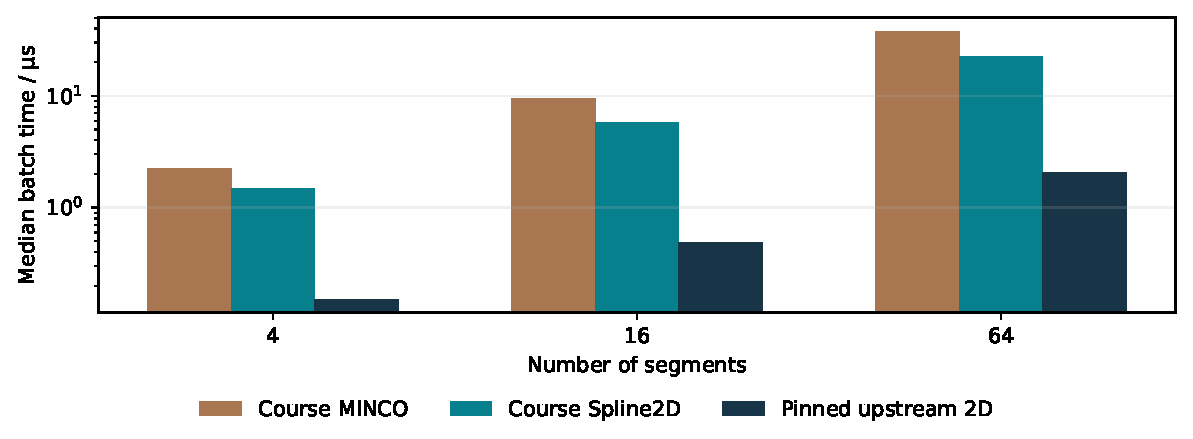
\includegraphics[width=\linewidth]{figures/ch16_comparison.pdf}
\caption{同一进程、相同输入下的构造、能量及完整能量梯度总耗时；纵轴为对数。
不包含地图、碰撞检查、I/O、ROS 或外层非线性优化。}
\end{figure}

\begin{center}\small
\begin{tabular}{rrrr}\toprule
段数 & 教学 MINCO/$\mu$s & 教学 Spline2D/$\mu$s & 固定上游/$\mu$s\\\midrule
4 & 2.247 & 1.476 & 0.152\\
16 & 9.453 & 5.793 & 0.484\\
64 & 38.000 & 22.735 & 2.049\\\bottomrule
\end{tabular}
\end{center}
GCC 15.2、Eigen 3.4、C++17，统一 -O3、-fno-fast-math，无 LTO；预热 10 次，21 组各 20 次，取组均值中位数。
同问题系数相对误差低于 $4.2\times10^{-14}$，能量梯度低于 $6.5\times10^{-13}$。
教学实现保留较多矩阵运算便于阅读；上游采用专门化公式。本机小实验不能替代完整规划器基准，也不承诺固定加速比。

\begin{enumerate}
\item \textbf{理解：}两种实现消去了不同变量，为何仍得到同一条曲线？
\item \textbf{代码 ch16-1：}补全 Schur 块，和独立 $4\times4$ 密集方程的解比较。
\item \textbf{实验：}改变段数与时长尺度，同时报告数值误差、失败状态及耗时，禁止只展示更快的一次。
\end{enumerate}
